\documentclass{article}
\usepackage{amsmath}
\title{Manual of coolpkg}
\author{John Doe}
\usepackage{Sweave}
\begin{document}
\Sconcordance{concordance:examp2.tex:examp2.Rnw:%
1 4 1 1 0 6 1 1 2 1 0 1 1 11 0 1 3 1 0 1 1 4 0 2 2 1 0 1 1 4 0 1 2 2 1}

\maketitle
\section{Introduction}
Some introduction to my coolpkg.
\section{Results}
Some data analysis results. Below is an example of the lm function.
\begin{Schunk}
\begin{Sinput}
> my.lm = lm(mpg~wt, data=mtcars)
> print(my.lm)
\end{Sinput}
\begin{Soutput}
Call:
lm(formula = mpg ~ wt, data = mtcars)

Coefficients:
(Intercept)           wt  
      37.29        -5.34  
\end{Soutput}
\end{Schunk}
\begin{Schunk}
\begin{Sinput}
> par(mfrow=c(2,2))
> plot(my.lm)
\end{Sinput}
\end{Schunk}
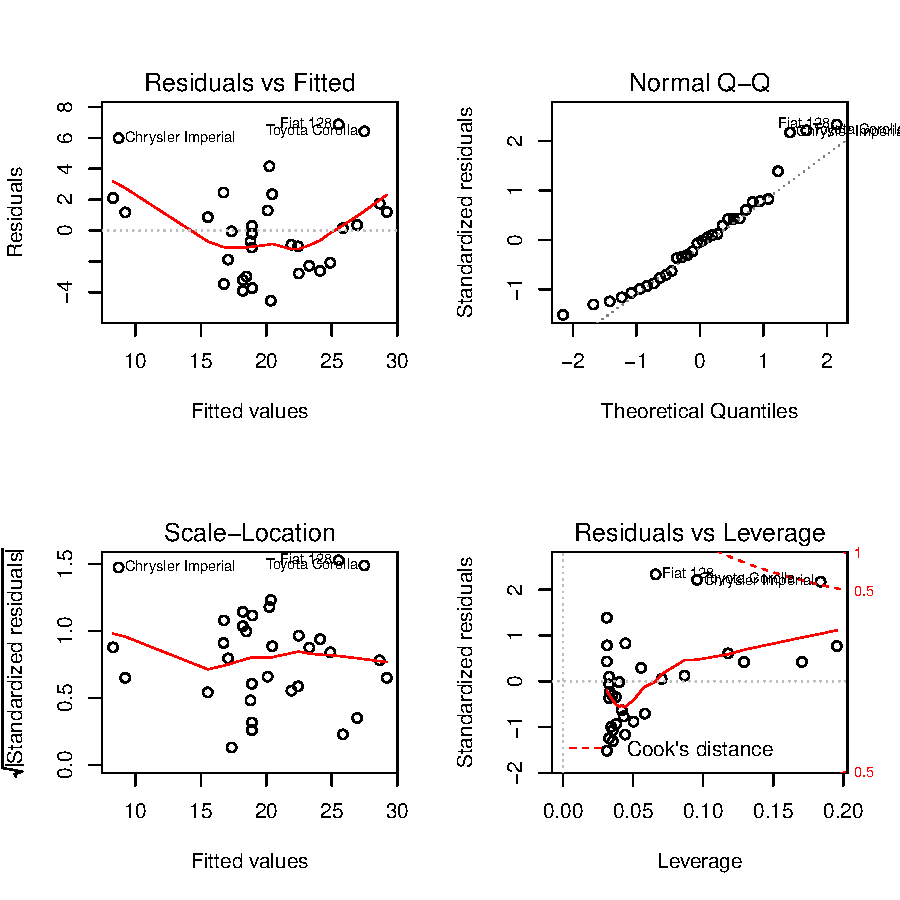
\includegraphics{examp2-002}

\begin{Schunk}
\begin{Sinput}
> par(mfrow=c(1,1))
> plot(mtcars$wt,mtcars$mpg)
\end{Sinput}
\end{Schunk}
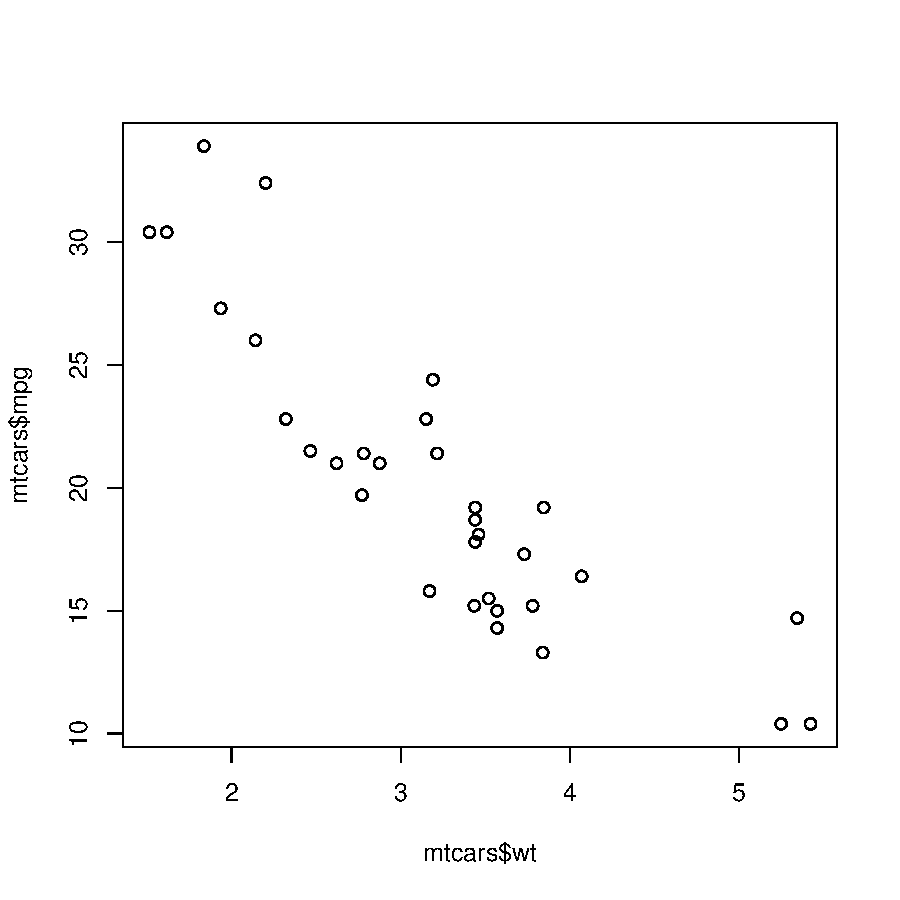
\includegraphics{examp2-003}
\section{Conclusion}
Conclusion texts are here.
\end{document} 
